\documentclass[10pt]{report}
%\usepackage{html}
\usepackage{graphicx}
\usepackage{algorithm,algorithmic}
\usepackage{Srcltx}
\usepackage{amsmath, amssymb, latexsym}
\usepackage{subfigure}
\renewcommand{\algorithmiccomment}[1]{{\it /* #1 */}}
\newcommand{\alglabel}[1]{\newcounter{#1}\setcounter{#1}{\value{ALC@line}}}
\newcommand{\algref}[1]{\arabic{#1}}
%%%%%%%%%%%%%%%%%%%%%%%%%
\setlength{\textheight}{8in}
\setlength{\textwidth}{5.2in}
\setlength{\topmargin}{-.15in}
%\addtolength{\oddsidemargin}{+0.2in}
\pagestyle{plain}
%\addtolength{\textheight}{+0.95in}
%%%%%%%%%%%%%%%%%%%%%%%%%%%%%%%%%
%Haixun's packages
%\newcommand\bnf[1]{$\langle$#1$\rangle$}
\newcommand\bnf[1]{#1}
\newcommand\exa[1]{\nopagebreak \begin{flushleft}\smallskip \nopagebreak
                \begin{minipage}[t]{#1}\sloppy}
\newcommand\exb[1]{\end{minipage}\kern 1cm\begin{minipage}[t]{#1}\sloppy }
\newcommand\exc{\end{minipage}\kern -3cm \smallskip\end{flushleft}}
\newcommand\oben[1]{\begin{center}\begin{minipage}{#1}\hrule\medskip}
\newcommand\unten  {\vspace{-.4cm}\hrule \end{minipage}\end{center}}
\newcommand\share[1]{\raisebox{1.5ex}[0pt]{#1}}
%%%%%%%%%%%%%%%%%%%from KDD%%%%%%%%%%%%%%%%%%%%%%%%%%%%
\newtheorem{theorem}{Theorem} \newtheorem{lemma}[theorem]{Lemma}
\newtheorem{claim}[theorem]{Claim}
\newtheorem{proposition}[theorem]{Proposition}
\newtheorem{corollary}[theorem]{Corollary}
\newtheorem{example}{Example}
\newtheorem{definition}{Definition}
\def\inv{\vspace*{-0.2cm}} %\def\back{\hspace*{-2cm}}
\def\pinv{\vspace*{0.2cm}}
\def\newdef#1{\emph{#1}}
%---------------------------------------------------------
\def\cdf{\sf} %Note: < and > are not in this font; use $<$ and $>$
\def\kw#1{\tt #1}
\def\cw{\small \tt }
\def\bw{\small \tt}
%
\newenvironment{codedisplay}
%{\renewcommand{\baselinestretch}{1}
{\vspace{-\partopsep}\cdf\addtolength{\baselineskip}{-1pt}
\samepage  \begin{tabbing} \quad
%\ \ \ \ \ \ \ \ \=\ \ \ \ \ \ \ \ \=\ \ \ \ \ \ \ \ \=\ \ \ \ \ \ \ \ \=
%\ \ \ \ \ \ \ \ \=\ \ \ \ \ \ \ \ \=\ \ \ \ \ \ \ \ \=\ \ \ \ \ \ \ \ \=
\ \ \ \ \=\ \ \ \ \=\ \ \ \ \=\ \ \ \ \= \ \ \=\ \ \ \
\=\ \ \ \ \=\ \ \ \ \= \ \ \=\ \ \ \ \=\ \ \ \ \=\ \ \ \ \=
\kill}
{\end{tabbing}\vspace{-\partopsep}\vspace{-\topsep}%\vspace{-\parsep}
}

\title{\Huge \bf The ATLaS User Manual \\}
\author{\Large Haixun Wang \\[0.1cm] \Large Carlo Zaniolo \\[0.1cm]\Large Richard Luo}

\begin{document}
\maketitle

%\renewcommand{\baselinestretch}{1.1}
\tableofcontents


\chapter{Introduction}

ATLaS is an SQL-based programming language for data-intensive applications.
Unlike languages, such as PL/SQL  or SQL/PSM, which use the imperative the constructs of
procedural languages, ATLaS achieves Turing completeness by using declarations, i.e.,
by supporting the declarations of new  aggregates and table functions.

An ATLaS program consists of list of declarations followed by a list of
SQL statements. Therefore, (with
{\tt A|B} denoting either {\tt A} or {\tt B}, and {\tt A*}
denoting zero or more occurrence of {\tt A}) we have:
%{\renewcommand{\baselinestretch}{1}
\begin{figure}[!htp]
\centering
\framebox{
\begin{tabular}{rll}
   \bnf{ATLaS-program} &$\rightarrow$& \bnf{ATLaS-dcl}$*$\;  \bnf{SQL-statement}$*$\\
  \bnf{ATLaS-dcl}     &$\rightarrow$&  \bnf{Table-dcl} $|$ \bnf{UDA-dcl} $|$ \bnf{TFunc-dcl} \\
  \end{tabular}
}
\caption{Syntax of ATLaS extensions \label{tab:syntax}}
\end{figure}

%}

The SQL-statements  mentioned  in Figure \ref{tab:syntax}
are the  basic select, insert, delete, update commands of
SQL-2,  which are summarized in Figure \ref{table:sql}.
We will assume that our reader is  already familiar with SQL-2 and
concentrate on the extensions which make
makes ATLaS so powerful.  ATLaS is Turing-complete
because of its declarations,
which are of three kinds:

\begin{enumerate}
\item  Table declarations (Table-dcl]),

\item  declarations of User-Defined Aggregates (UDA-dcl),

\item  declarations of Table Functions (TFunc-dcl).
\end{enumerate}

In the next  Section  we discuss simple programs that only use table
declarations. Programs
containing user-defined aggregates and table functions are
discussed in  the following sections.

\chapter{ATLaS SQL on Tables}
ATLaS can use a variety of tables from different sources. In
particular, it can access B+Tree indexed tables managed by the embedded
database system Berkeley DB~\cite{berkeleydb}. For instance, say that an
employee table, with key $\tt Eno$, is stored in such a format in
the directory\\
$\tt C$:$\tt \backslash mydb \backslash employees$.
[Say more about win vs linux] Then the following
program  first gives a 5 \% raise to the employees in the 'QA'
department, and then prints all the employees who now make more
than 60K:


\begin{codedisplay}
\tt
\>\>\>\>\>\>\>\>\> $\slash$* Begin of ATlaS program--- this is a comment*$\slash$\\
\>\>table employees(Eno int, Name char(18), Sal real, Dept char(6)) \\
 \> \>    \> \> \> \> Btree(Eno) ~  source \
 '$\tt C$:$\tt \backslash  mydb\backslash employees$';\\[0.1cm]
 \> \> update employees set Sal = Sal * 1.05\\
       \> \> \> \> \> where Dept='QA' ;\\[0.1cm]
 \> \> insert into stdout select Eno, Name\\
 \> \> \> \> \> from employees where Sal $>$ 60000;\\
\>\>\>\>\>\>\>\>\> $\slash$* End of ATlaS program *$\slash$\\
\end{codedisplay}

The {\tt insert into stdout} clause before {\tt select} in the last
statement can be omitted without changing the meaning of this program.
Thus ATLaS supports the standard {\tt select, insert, delete, update}
statements of SQL-2. Observe that keywords can be written in upper
case or lower case---however, attribute names and other user-defined
identifiers are case-sensitive.

Since we assume that our readers are already familiar
with SQL-2, we will now concentrate on the new constructs of ATLaS and
return to SQL in Section 6.

Three types of tables are currently supported in ATLaS, as follows:

\begin{enumerate}
\item Secondary storage tables with indexed by B+ trees on one or more attributes,
as in the following example:

\begin{codedisplay}
\tt
\>\> TABLE employees(Eno int, Name char(18), Sal real, Dept char(6)) \\
 \> \>  \> \> \> \> BTree(Eno)
 source '$\tt C$:$\tt \backslash  mydb \backslash employees$';\\
\end{codedisplay}

The  $\tt SOURCE$ declaration associates this table with the file
$\tt C$:$\tt \backslash  mydb \backslash employees$ and make it
 {\em persistent}. Persistent tables remain after
the the program completes its execution. Tables declared without a $\tt source$
are {\em transitory} and they are removed at the end of the program
execution.

\item Secondary storage tables with indexed by R+ trees on a pair
or a quadruplet of real attributes: the first can be
used to index points, and the second for rectangles:

\begin{codedisplay}
\tt
\>TABLE mypoints(x real, y real, object char(10)) RTree(x,y); \\[0.2cm]

\> TABLE myrectangles(tx real, ty real, bx real, by real, object char(10))\\
  \> \>  \> \> \> \>      \> \>  \> \> \> \>     RTree(tx,ty,bx,by);
\end{codedisplay}
\item
Main memory tables, with a hash-based index on one or more
attributes:
\begin{codedisplay}
\tt
TABLE memo(j Int,  Region Char(20))\\
\>\>\> MEMORY AS VALUES(0, `root-of-tree`);
\end{codedisplay}
This example also illustrates that a transitory
table can be  initialized to the results of the query defined using the
{\tt AS query} option. In this example, we use constant values to
initialize the table. In general, the initialization query can
use the content of previously declared tables.
\end{enumerate}
A source declaration can only be given for B+tree and R+tree tables, but not for
{\tt MEMORY} tables since these are never persistent.
The syntax of table declarations is as follows:


\begin{table}[!htp]
\centering
\framebox{
\begin{tabular}{rll}
    \bnf{Table-dcl} &$\rightarrow$ & `TABLE` ~ \bnf{table-id}
`(` \bnf{columns} \bnf{keydec} `)`\\
     & &~~~~~~~~~~ [`SOURCE` $|$ `$'$`\bnf{file-name}`$'$``AS` \bnf{query}] `;`\\
    \bnf{column-list} &$\rightarrow$& \bnf{column} [`,`  \bnf{column}]* \\
    \bnf{column} &$\rightarrow$& \bnf{id} \bnf{type} \\
    \bnf{type} &$\rightarrow$& `INT` $|$ `REAL` $|$ `CHAR` `(` \bnf{num} `)` $|$  `REF` `(` \bnf{id} `)`\\
    \bnf{keydec} &$\rightarrow$& [`BTree(`\bnf{key}`)`, `RTree(`\bnf{key}`)`, MEMORY] `;`\\
  \bnf{key} &$\rightarrow$&  `(` \bnf{id} [`,` \bnf{id}]* `)` \\
 \\
 \bnf{load} &$\rightarrow$& `LOAD` \ `FROM` `$'$`\bnf{file-name}`$'$` `INTO` \bnf{table-id}\\

  \end{tabular}
}
\caption{Declaring and Initializing Tables in ATLaS.}
\end{table}
The {\tt LOAD} construct of ATLaS  can be used to load into a table data from
an external file, where the commas (carriage returns) are used as separators
between attribute values (records). Newly loaded tuples are appended to
the existing tuples.


%Here we summarize the subset of standard SQL supported in ATLaS:
\begin{table}[!hb]
\renewcommand{\baselinestretch}{0.9}
\centering
{\bf SQL Statements}\\[0.2cm]
\framebox{
\begin{tabular}{rll}
    \bnf{SQL-statement} &$\rightarrow$&  \bnf{select-st}$|$
    \bnf{delete-st}$|$ \bnf{insert-st}$|$ \bnf{update-st}\\[0.1cm]
%\\
    \bnf{select-st} &$\rightarrow$&  \bnf{query} [\bnf{order-clause}] `;` \\
    \bnf{order-clause} &$\rightarrow$& `ORDER` \ `BY` \bnf{exp} [`ASC` $|$ `DSC`]
    [`,` \bnf{exp} [`ASC` $|$ `DSC`]]*\\
    \bnf{query}  &$\rightarrow$& \bnf{query-block} [\bnf{set-op} \bnf{query-block}]*\\
 \bnf{set-op}  &$\rightarrow$&  `UNION`$|$`INTERSECT`$|$`EXCEPT` \\[0.1cm]
    \bnf{query-block} &$\rightarrow$& `SELECT` \bnf{hxp} [, \bnf{hxp}]* \\
    && `FROM` \bnf{squn} [`,` \bnf{squn}]* \\
    && [`WHERE` \bnf{exp}] \\
    && [`GROUP` \ `BY` \bnf{exp} [`,` \bnf{exp}]* \\
    && [`HAVING` \bnf{exp}] \\[0.1cm]
    \bnf{delete} &$\rightarrow$& `DELETE` \ `FROM` \bnf{id} [`WHERE` \bnf{exp}] `;` \\
    \bnf{insert} &$\rightarrow$& `INSERT` \ `INTO` \bnf{id} \bnf{select-st} `;`\\
    & & VALUE ... not defined?\\
    \bnf{update} &$\rightarrow$& `UPDATE` \bnf{id} `SET` \bnf{update-list} [`WHERE` \bnf{exp}] `;` \\
    \bnf{update-list} &$\rightarrow$& \bnf{id} `=` \bnf{exp} [`,` \bnf{id} `=` \bnf{exp}]*\\[0.1cm]
%\end{tabular}
%\begin{tabular}{rll}
    \bnf{exp} &$\rightarrow$& `NIL`
 $|$ \bnf{num}
$|$ \bnf{float}
$|$ \bnf{string}
$|$ \bnf{id} [ `.` \bnf{id}]
 $|$ \bnf{ref}\\
 %&& $|$ \bnf{exp} (`+`$|$`-`$|$`*`$|$`/`$|$`  \\
    && $|$ \bnf{exp} (`=`$|$` $<$ `$|$` $<=$`$|$`$>$`$|$`$>=$ `$|$`$<>$`) \bnf{exp}\\
    && $|$ \bnf{exp} (`AND`$|$`OR`$|$`IN`$|$`NOT`\ `IN`) \bnf{exp}\\
    && $|$ `EXISTS` \bnf{exp}\\
    && $|$ (`max`$|$`min`$|$`count`$|$`sum`$|$`avg`) `(`\bnf{exp}`)`\\
   % && $|$ \bnf{udf} [ `$\rightarrow$` \bnf{id}]\\
%    && $|$ \bnf{case-exp}\\
    && $|$ `(` \bnf{exp} `)`\\
    && $|$ `(` \bnf{query} `)`\\
    %&& $|$ `{` {@ \bnf{vdec}} {@ \bnf{exp} `;`} `}` \\
  \bnf{ref} &$\rightarrow$& \bnf{ref} `$\rightarrow$` \bnf{id}
 $|$ \bnf{id} [`.` \bnf{id}] `$\rightarrow$` \bnf{id}\\[0.1cm]
% \end{tabular}
%\begin{tabular}{rll}
 %\bnf{case-exp} &$\rightarrow$& `CASE` \bnf{exp} \bnf{when-exp-list} [`ELSE` \bnf{exp}] `END`\\
 %   && $|$ `CASE` \bnf{when-exp-list}  [`ELSE` \bnf{exp}] `END`\\
 %   \bnf{when-exp-list} &$\rightarrow$& `WHEN` \bnf{exp} `THEN` \bnf{exp}
%[`WHEN` \bnf{exp} `THEN` \bnf{exp}]*\\
    \bnf{id} &$\rightarrow$& \bnf{letter} [\bnf{letter} $|$ \bnf{digit}]* \\
    \bnf{letter} &$\rightarrow$& (`a`-`z`$|$`A`-`Z`)\\
    \bnf{digit} &$\rightarrow$& (`0`-`9`)\\[0.1cm]
%\\
    \bnf{hxp} &$\rightarrow$& \bnf{exp} [[`AS`] \bnf{hxp-alias}] $|$ [\bnf{id} `.`] `*`\\
    \bnf{hxp-alias} &$\rightarrow$& \bnf{id} $|$ `(` \bnf{id} [`,` \bnf{id}]* `)`\\
    \bnf{qun-alias} &$\rightarrow$& [`AS`] \bnf{id} [`(` \bnf{id} {@ `,` \bnf{id}} `)`]\\[0.1cm]
    %\bnf{udf} &$\rightarrow$& \bnf{id} `(` [\bnf{exp} {@ `,` \bnf{exp}}] `)`\\
%\\
%    \bnf{case-exp} &$\rightarrow$& `CASE` \bnf{exp} \bnf{when-exp-list} [`ELSE` \bnf{exp}] `END`\\
%    && $|$ `CASE` \bnf{when-exp-list}  [`ELSE` \bnf{exp}] `END`\\
%    \bnf{when-exp-list} &$\rightarrow$& `WHEN` \bnf{exp} `THEN` \bnf{exp} {@ `WHEN` \bnf{exp} `THEN` \bnf{exp}}\\
%    \bnf{id} &$\rightarrow$& \bnf{letter} {@ \bnf{letter} $|$ \bnf{digit}}\\
  \end{tabular}
  }
\caption{Syntax of the basic SQL Statements supported in ATLaS} \label{table:sql}
\end{table}

\chapter{User-Defined Aggregates}
ATLaS supports the standard five aggregates {\tt count, sum,
avg, min}, and {\tt max} without the {\tt DISTINCT} option.
But the real power of ATLaS follows from its User-Defined Aggregates
(UDAs) discussed next.
As a first example, we define an aggregate equivalent to the standard
{\bw avg} aggregate in SQL.
\paragraph{Standard Average} The first
line of this aggregate function declares a local table, {\tt
state}, to keep the sum and count of the values processed so far.
While, for this particular example, {\bw state} contains only one
tuple, it is in fact a table that can be queried and updated using
SQL statements and can contain any number of tuples (see later
examples). These SQL statements are grouped into the three blocks
labelled respectively {\cw INITIALIZE}, {\cw ITERATE}, and {\cw
TERMINATE}. To compute the average, the SQL statement in
{\cw INITIALIZE} inserts the value taken from
the input stream and sets the count to $1$. The {\cw ITERATE}
statement updates the table by adding the new input value to the
sum and $1$ to the count. The {\cw TERMINATE} statement returns
the final result(s) of computation by {\cw INSERT INTO RETURN} (to
conform to SQL syntax, {\cw RETURN} is treated as a virtual table;
however, it is not a stored table and cannot be
used in any other role): \\

\begin{codedisplay}
\tt
\> AGGREGATE myavg(Next \kw{Int}) : Real\\
\>\{\> {TABLE} state(sum \kw{Int}, cnt \kw{Int}); \\
\>\> {INITIALIZE} : \{\\
\>\>\>INSERT INTO state {VALUES} (Next, 1);\\
\>\>\}\\
\>\>\ {ITERATE} : \{\\
\>\>\>{UPDATE} state {SET} sum=sum+Next, cnt=cnt+1;\\
%\>\>\kw{INSERT} \kw{INTO} \kw{RETURN} \\
%\>\>\>\kw{SELECT} sum/cnt \kw{FROM} state\\
%\>\>\>\kw{WHERE} cnt \% 100 = 0;\\
\>\>\}\\
\>\>{TERMINATE} : \{\\
\>\>\>{INSERT} {INTO} {RETURN} {SELECT} sum/cnt {FROM} state;\\
\>\>\}\> \\
\>\}\\
\end{codedisplay}

The basic initialize-iterate-terminate template used to define the
average aggregate of SQL-2, can now be used to defined powerful
new aggregates required by new database applications.

\paragraph{OnLine Average}For instance, there is much current interest in online
aggregates~\cite{hellerstein}. Since averages converge toward the correct
value well before all the tuples in the set have been visited, we
can have an online aggregate that returns the average-so-far
every, say, 200 input tuples. (In this way, the user or the
calling application can stop the computation as soon as
convergence is detected.) Online averages can be expressed in
ATLaS as follows:

\begin{codedisplay}
\>\kw{AGGREGATE} online\_avg(Next \kw{Int}) : \kw{Real}\\
\>\{\>\kw{TABLE} state(sum \kw{Int}, cnt \kw{Int}); \\
\>\> \kw{INITIALIZE} : \{ \\
\>\>\> \kw{INSERT INTO} state \kw{VALUES} (Next, 1);\\
\> \> \} \\
\>\> \kw{ITERATE}: \{ \\
\>\>\> \kw{UPDATE} state \kw{SET} sum=sum+Next, cnt=cnt+1;\\
\>\>\>\kw{INSERT} \kw {INTO} \kw{RETURN} \\
\>\> \> \kw{SELECT} sum/cnt \kw{FROM} state \kw{WHERE} cnt \% 200 = 0; \\
\>\>\}\\
\>\>\kw{TERMINATE} : \{  \ \}\\
\>\}\\
\end{codedisplay}

Therefore, the online average program has been obtained from the
traditional average program by removing the statements from
{\cw{TERMINATE}} and adding a {\cw{RETURN}} statement to
{\cw{ITERATE}}.  Our UDA {\bw {online\_avg}} takes a
stream of values as input and returns a stream of values as output
(one every 200 tuples). In this example only one tuple is
added to output by the  the {\small
{INSER INTO RETURN}} statement; in general, however, such statement can produce
(a stream of) several tuples. Thus ATLaS UDAs operate as
general stream transformers.

ATLaS uses the same basic framework to define both traditional
aggregates and non-blocking aggregates. ATLaS UDAs are non-blocking
when their {\cw{TERMINATE}} clause is either empty or absent.

The typical default
semantics for SQL aggregates is that the data is first sorted
according to the {\cw GROUP-BY} attributes; this is
a blocking operation.  However, ATLaS's default
semantics for UDAs is that the data is pipelined through the
{\cw INITIALIZE} and {\cw ITERATE} clauses where the input stream is transformed
into the output stream: the only blocking operations (if any) are
those specified in {\cw TERMINATE}, and only take place at the end of the
computation.


\paragraph{Calling User-Defined Aggregates (UDAs)} UDAs are called as any other builtin aggregate.  For instance,
given a database table {\tt {employee(Eno, Name, Sex, Dept,
Sal)}}, the following statement computes the average salary of
employees in department 1024 by their gender:


\begin{codedisplay}
\>\>\>\>\>\>\kw{SELECT} Sex, online\_avg(Sal)\\
\>\>\>\>\>\>\kw{FROM} employee \kw{WHERE} Dept=1024 \kw{GROUP BY}
Sex;\\
\end{codedisplay}


Thus the results of the selection, defined by {\bw Dept= 1024}, are pipelined to
the aggregate in a stream-like fashion.

\paragraph{SQLCODE}
This a convenient labor-saving device found in most
SQL systems, that comes very
handy for the ATLaS programmer who
wants to correlate a statement with
the next. SQLCODE is set to a positive value when the last
statement had a null effect, and to zero otherwise.
Thus to tell the user that no
employee was found in department $\tt 1024$, we can modify the previous
program as follows:


\begin{codedisplay}
\tt
\>\>\>\>\>\>\kw{SELECT} Sex, online\_avg(Sal)\\
\>\>\>\>\>\>\kw{FROM} employee \kw{WHERE} Dept=1024 \kw{GROUP BY}
Sex;\\
\>\>\>\>\>\>select 'Nobody found in that department'\\
\> \> \> \> \>  \> \> \> \> \>where SQLCODE $>$0;\\
\end{codedisplay}
In the last statement, the predicates in the $\tt WHERE$ clause controls its
conditional execution, in a fashion similar to that of the $\tt IF$ clauses in
a procedural programming language. In fact, the  ATLaS compiler recognizes,
and optimizes execution of, such conditional predicates.

\paragraph{Minima: Points and Values.} In the next Example, we have
a sequence of point-value pairs, and
we  define a {\bw minpair} aggregate
that returns the point where a minimum occurs
along with its value at the minimum.


\begin{codedisplay}
\kw{AGGREGATE} minpair(iPoint \kw{Int}, iValue \kw{Int}): (mPoint \kw{Int}, mValue \kw{Int})\\
 \{ \>  \kw{TABLE} mvalue(value \kw{Int}) MEMORY;
 \kw{TABLE} mpoints(point \kw{Int}) MEMORY; \\
\>\kw{INITIALIZE}: \{ \\
\>\> \kw{INSERT} \kw{INTO} mvalue \kw{VALUES} (iValue);\\
\>\> \kw{INSERT} \kw{INTO} mpoints \kw{VALUES}(iPoint);\\
\> \} \\
\>\kw{ITERATE}: \{\\
\>\> \kw{UPDATE} mvalue \kw{SET} value = iValue \kw{WHERE} iValue $<$ value;\\
\>\> \kw{DELETE FROM} mpoints \kw{WHERE} SQLCODE = 0;\\
% \>\>\kw{INSERT} \kw{INTO} mpoints \\
% \>\>\>\> \kw{SELECT} iPoint \kw{FROM} mvalue\\
% \>\>\>\> \kw{WHERE}  iValue $=$mvalue.value;\\
 \>\>\kw{INSERT} \kw{INTO} mpoints \kw{SELECT} iPoint \kw{FROM} mvalue\\
 \>\>\> \>\>\>\>\>\>\>\>\kw{WHERE}  iValue $=$mvalue.value;\\
\> \} \>\>\>\>\>\>\>\>\\
%
\>\kw{TERMINATE}: \{ \\
\>\>\kw{INSERT} \kw{INTO} \kw{RETURN} \kw{SELECT} point, value \kw{FROM} mpoints, mvalue;\\
\> \}  \\
\}\\
\end{codedisplay}

Here have used two internal tables: the {\bw mvalue} table holds, as its only entry,
the current min value, while {\bw points} holds all the points where this
value occurs.
In the {\small \kw{ITERATE}} statement we have used {\cw {SQLCODE}}
to `remember' if the previous statement updated {\bw mvalue}; this is the situation in which
the old value was larger than the new one and the old points
must be discarded.

Then, the last statement in {\cw ITERATE}
adds the new {\bw iPoint} to {\bw mpoints} if the
input value is equal to the current min value. In the UDA
definition the formal parameters of the UDA function are treated
as constants in the SQL statements. Thus, this third
{\cw INSERT} statement adds the constant value of {\bw iPoint}
to the {\bw mpoints} relation, provided that {\bw iValue} is the
same as the value
in {\bw mvalue}---thus the {\cw FROM} and {\cw WHERE} clauses
operate here as conditionals.
The {\cw RETURN} statement returns the final list of min pairs as a stream.

For instance, say that we have a time series containing the daily  closing
prices of certain stocks arranged in temporal sequence (i.e. the table {\tt stock\_prices},
below). Then the following program computes the local minima for each stock:

\begin{codedisplay}
\> /* The declaration of {AGGREGATE} minpair  should go here*/\\
\> TABLE stock\_prices(Day Int, Stock char(4), Cprice Real)\\
\hspace{6cm}source  'D:$\backslash$mydabase$\backslash$stock\_prices'\\

%\>\>insert into stdout\\
\>\>select Stock, minpair(Day, Stock) $\rightarrow$ iPoint, minpair(Day, Stock)$\rightarrow$  iValue \\
\>\>from stock\_prices\\
\>\>group by Stock  ordered by Stock, minpair(Day, Stock) $\rightarrow$ iPoint\\
\end{codedisplay}

Observe the use of  ``$\tt \rightarrow$" to identify the different
components in the two-column tuples returned by the aggregate $\tt minpair$.
Since temporal data types are not yet supported
in the current ATLaS version,
we are using integers to represent dates:
thus May, 27, 1999 is represented as {\tt 19990527}.

The next table summarizes the syntax for declaring new aggregates.

\begin{figure}[!htp]
\centering
\framebox{
\begin{tabular}{rll}
    \bnf{UDA-dcl} &$\rightarrow$& `AGGREGATE` \bnf{id} `(` \bnf{column-list} `)` `:`
             \bnf{return-type} \bnf{aggr-body}\\
    \bnf{aggr-body} &$\rightarrow$& `\{` \bnf{ATLaS-dcl*} \\
      && \ \ \ `INITIALIZE` \ `:` \{  \bnf{SQL-statement*} `;`\}` \\
      && \ \ \ `ITERATE` \ `:` \{ \bnf{SQL-statement*} `;`  `\}` \\
      && \ \ \ `TERMINATE` \ `:` \{ \bnf{SQL-statement*} `;`\}` \\
    && `\}` \\
    \bnf{return-type} &$\rightarrow$& \bnf{type} $|$ `(` \bnf{column-list} `)`\\
\end{tabular}
}
\caption{The declaration of UDAs}
\end{figure}


\paragraph{Initializing Tables and Combining Blocks.}
Let us now introduce  the following two syntactic variations of
convenience supported in ATLaS:
\begin{itemize}
\inv \item Tables declared in UDAs can be initialized as part of their declaration,
via an SQL statement. This executes at the time when the first tuple is
processed, thus the result is the same as if the initialization had
been executed in the {\small INITIALIZE} block.

\inv \item Different blocks can be merged together when they perform the
same function. In the next example the {\small INITIALIZE}
and {\small ITERATE} blocks are merged together.
\end{itemize}
Our  Online Averages UDA could also have been written as follows:
\begin{codedisplay}
\>\kw{AGGREGATE} online\_avg(Next \kw{Int}) : \kw{Real}\\
\>\{\>\kw{TABLE} state(sum \kw{Int}, cnt \kw{Int}) AS VALUES(0, 0); \\
\>\> \kw{INITIALIZE}:\kw{ITERATE}:  \{ \\
\>\>\> \kw{UPDATE} state \kw{SET} sum=sum+Next, cnt=cnt+1;\\
\>\>\>\kw{INSERT} \kw {INTO} \kw{RETURN} \\
\>\> \> \kw{SELECT} sum/cnt \kw{FROM} state \kw{WHERE} cnt \% 200 = 0; \\
\>\>\}\\
\>\}
\end{codedisplay}

In the previous example,
the  statement has been
omitted: this is equivalent to writing
 `{\cw{TERMINATE: \{ \} }}'. An empty {\kw{INITIALIZE}}
statement can also be omitted in a similar fashion.

The results produced by online averages depend
on the order in which the data is streamed through the UDA.
This illustrate a common situation in stream processing:
the  abstract semantics of the aggregate used is
order-independent, but approximations must be used
because of efficiency and real-time requirements (e.g., nonblocking
computations); often, the approximate UDA is order-dependent.

In other situations, no approximation is involved, and the
dependence on order follows from the very semantics of the UDA.
For instance, this is the case of the {\tt rising aggregate} described below.
\paragraph{Rising.} In addition to temporal extensions of standard
aggregates (suggested homework: write them in ATLaS),
TSQL2~\cite{ads}
proposes this new aggregate to return the maximal time periods during
which a certain attribute values has been increasing monotonically.
We can apply this aggregate to our
{\cdf stock\_prices(Day Int, Stock char(4), Cprice Real)} table to find
the periods during which different stocks have been rising, as follows:

\begin{codedisplay}
%\>\>insert into stdout\\
\>\>select Stock, rising(Day, Cprice) $\rightarrow$ Start,
rising(Day, Cprice)$\rightarrow$ End\\
\>\>from stock\_prices\\
\>\>group by Stock \\
\end{codedisplay}
where {\tt rising} is defined as follows:


\begin{codedisplay}
\>AGGREGATE rising(iPoint Int, iValue Real) : (Start Int, End Int)\\
\> \{ TABLE rperiod(First Int, Last Int, Value Real) MEMORY;\\
 \>\> INITIALIZE: \{ \\
\>\> \>\>  INSERT INTO rperiod VALUES (iPoint, iPoint, iValue);\\
 \>\>\> \}\\
\>\>ITERATE: \{ \\
\>\> \>\>            INSERT INTO return SELECT First, Last\\
\>\> \>\>   \>\>          FROM rperiod\\
\>\> \>\>   \>\>         WHERE  iValue $<$= Value AND First $<$ Last;\\
\>\> \>\>        UPDATE rperiod SET Last=iPoint, Value=iValue\\
\>\> \>\>   \>\>           WHERE iValue $>$  Value; \\
\>\> \>\> UPDATE rperiod SET First=iPoint, Last=iPoint, Value=iValue\\
 \>\> \>\>    \>\>              WHERE SQLCODE $>$ 0;\\
  \>\>\> \} \\

 \>\>TERMINATE:\{ INSERT INTO return SELECT First, Last \\
   \>\> \>\>   \>\>           FROM rperiod \\
     \>\> \>\>   \>\>             WHERE   First $<$ Last; \}\\
  \>\>\> \}\\
\> \}
\end{codedisplay}

Therefore we have a sequence of time-value ordered by increasing
time. We store a zero length period {\tt iPoint, iPoint} whenever
the new {\tt iValue} is not increasing (also at
{\tt INITIALIZE}). Also a non-zero length period is currently
held in {\tt rperiod} we  return it.
When the new {\tt iValue} is larger than the
previous stored value, we advance the {\tt End} of the current
period to the current point.


\chapter{Table Functions}
Table functions play a critical role in rearranging data, and
allowing the composition of aggregates. For instance,
if we want to count the number
of the local minima found in the execution of {\tt minpair},
we can use the following table function:


\paragraph{Cascading of Aggregates via a Tfunction}
\begin{codedisplay}
\> /* include the declaration of the {AGGREGATE} minpair here*/\\
\> TABLE stock\_prices(Day Int, Stock char(4), Cprice Real)\\
\>\>\>\>\>\>\>\>\>\>\>source  'C:$\backslash$mydabase$\backslash$stock\_prices' ;\\

\>FUNCTION localmins():(Stock Int, Point Int, Value Int)\\
\>\> \{ \> insert into RETURN\\
\>\>\>select p.Stock, minpair(p.Day, p.Cprice)\\
\>\>\>\>from stock\_prices as p\\
\>\>\>\> group by p.Stock\\
\> \>\> \} \\[0.2cm]
\>select  L.Stock,  count(L.Point)\\
\>\>from  stock\_prices, TABLE(localmins()) AS L\\
\>\>group by L.Stock; \\
\>\\
\end{codedisplay}

Here the table function does little more than calling the {\tt minpair}
aggregate on the {\tt stock\_prices} table, and organizing the results
as a virtual table with attributes  {\tt (Stock, Point, Value)}. Then,
the aggregate {\tt count} can be called on this virtual table,
whereas the direct cascading of aggregates is not allowed in
SQL, nor in ATLaS.

Also observe that the notation
{\tt TABLE( ...)} must be used when invoking table functions,
to conform to SQL standards.

The final NB is that the `dot' notation
(e.g., {\tt L.Point})  is used to refer to the various columns in a
tuple produced by a table function, whereas we use``$\rightarrow$''
for UDAs (e.g., {\tt minpair(Day, Stock) $\rightarrow$ iPoint}).

\paragraph{Pre-Sorting the Data}
The correctness of the $\tt rising$ is predicated upon the data
being sorted by increasing time. If that is not the case, we can
use a table function to pre-sort the data. Then, our program
becomes:
\begin{codedisplay}
\> /*{AGGREGATE} minpair  include here the rising declaration*/\\
\> TABLE stock\_prices(Day Int, Stock char(4), Cprice Real)\\
\>\>\>\>\>\>\>\>\>\>\>source  'C:$\backslash$mydabase$\backslash$stock\_prices' ;\\[0.1cm]
\>FUNCTION sort():(Stock Int, Point Int, Value Int)\\
\>\> \{ \> insert into RETURN\\
\>\>\>select Day, Stock, Cprice)\\
\>\>\>\>from stock\_prices\\
\>\>\>\> ORDERED BY Stock, Day\\
\> \>\> \} \\[0.1cm]
\>\>insert into stdout\\
\>\>select Stock, rising(Day, Stock) $\rightarrow$ Start,
rising(Day, Stock)$\rightarrow$ End\\
\>\>from stock\_prices, TABLE(sort())\\
\>\>group by Stock\\
\end{codedisplay}


\paragraph{Column Value Pair}The first step for most scalable classifiers
is to convert the training set into column/value pairs. For instance,
say that our training set is as follows, where the  various conditions
are described by their initials (e.g., S, O, R in the first column stand
respectively for Sunny, Overcast, and Rain):

\begin{figure}[htb]
\begin{center}
{\footnotesize
\begin{tabular}{|c|c|c|c|c|c|} \hline
{\bf RID}&{\bf Outlook}&{\bf Temp}&{\bf Humidity}&{\bf Wind}&{\bf Play}\\
\hline
1&S&H&H&W&N\\
2&S&H&L&S&N\\
3&O&H&L&W&Y\\
4&R&M&H&W&Y\\
$\ldots$& $\ldots$& $\ldots$ & $\ldots$ & $\ldots$& $\ldots$\\
\end{tabular}
}
\caption{The relation \bf PlayTennis} \label{tab:tennis}
\end{center}
\end{figure}

Then, we want to convert {\bw PlayTennis} into a new
stream of three columns {\bw (Col, Value, YorN)} by breaking down each
tuple into four records, each record representing one column in the
original tuple, including the column number, column value and the
class label {\bw YorN}. For instance, the first tuple should
produce the following
tuples:

$$\tt
(1, S, N), \ (2, H, N), \ (3, H, N), \ (4, W, N)$$
Our next table function, called
{\tt dissemble}  can be used for the task.

\begin{codedisplay}
\kw{FUNCTION} dissemble\\
\> \>(v1 \kw{Char(1)}, v2 \kw{Char(1)}, v3 \kw{Char(1)},
v4 \kw{Char(1)}, YorN \kw{Char(1)}):\\
\> \>  \> \> \> \> \> \>\hspace{2cm}  (col \kw{Int}, val \kw{Char(1)}, YorN \kw{Char(1)}); \\
\> \{\kw{INSERT} \kw{INTO} \kw{RETURN}\\
 \> \> \> \kw{VALUES} (1, v1, YorN), (2, v2, YorN),\\
  \> \> \> \> \> \>\kw{}(3, v3, YorN), (4, v4, YorN);\\
 \> \> \}\\
\end{codedisplay}

\begin{figure}[hbt]
\centering
\framebox{
\begin{tabular}{rll}
    \bnf{Tfunc-dcl} &$\rightarrow$& `FUNCTION` \bnf{id} `(` \bnf{column-list} `)` `:`
             \bnf{return-type} \bnf{Tfunc-body} \\
  \bnf{return-type} &$\rightarrow$& \bnf{type} $|$ `(` \bnf{column-list} `)`\\
  \bnf{Tfunc-body} &$\rightarrow$& `\{` \bnf{ATLaS-dcl*}  \bnf{SQL-statement*} `\}` \\

\end{tabular}
}
\caption{The declaration of a Table Function}
\end{figure}
The syntax for function tables is given below.
 The mapping expressed by {\tt dissemble} could be expressed in standard
 SQL via the union of several statements, but such a formulation could
 lead to inefficient execution. In later sections we will show that,
using this table function and specialized aggregates we can
express Naive Bayesian classifiers and Decision Tree Classifiers in
a few ATLaS statements.

\chapter{Programming in ATLaS}
\section{Recursion}
Example \ref{exe:trc} illustrates the typical structure of an ATLaS
program. The declaration of the table {\bw dgraph(start, end)} is followed
by that of the UDA {{\bw reachable}}; the table and the UDA are then used
in an SQL statement that calls for the computation of all nodes reachable from
node {\bw '000'}. The clause {\cw SOURCE({\bw mydb})} denotes that
{\bw dgraph} is a table from a database that is known to
the systems by the name {\bw 'mydb'}. (Without the {\kw{SOURCE}} clause
{\bw dgraph} is local to the program and discarded once its execution
 completes).

The program of Example~\ref{exe:trc}
shows one way in which the transitive closure
of  a graph can be expressed in
ATLaS. We use the recursive UDA {{\bw reachable}}
that perform a depth-first traversal of the graph
by recursively calling itself.  Upon receiving a node,
{{\bw reachable}} returns the node
to the calling query along with all the nodes reachable from it.
(We assume that the graph contains no directed cycle;
otherwise a table will be needed to memorize
previous results and avoid
infinite loops.)
Observe that the {\cw INITIALIZE} and {\cw ITERATE} routine in
Example~\ref{exe:trc} share the same block of code.


\begin{example}{Computation of Transitive Closure\label{exe:trc} \pinv}

\begin{codedisplay}
\>\>\kw{TABLE} dgraph(start \kw{Char}(10), end \kw{Char}(10))  \kw{SOURCE} (mydb); \\[0.2CM]

\>\>\kw{AGGREGATE} reachable(Rnode \kw{Char}(10)) : \kw{Char}(10) \\
\>\>\{\> \kw{INITIALIZE}: \ \kw{ITERATE}: \{ \\
\>\>\>\> \kw{INSERT} \kw{INTO} \kw{RETURN} \kw{VALUES} (Rnode) \\
\>\>\>\>\kw{INSERT} \kw{INTO} \kw{RETURN} \\
\>\>\>\>\> \kw{SELECT} reachable(end) \kw{FROM} dgraph\\
\>\>\>\>\> \kw{WHERE}  start=Rnode;  \\
\>\>\>\}\\
\>\>\}\\
\>\>\kw{SELECT} reachable(dgraph.end) \kw{FROM} dgraph \\
\>\>\kw{WHERE} dgraph.start='000';
\end{codedisplay}

\end{example}

Besides the  Prolog-like top-down
computation of Example \ref{exe:trc}, we can also express easily the
bottom-up computation used in  Datalog,
and a stream-oriented computation will be discussed in the next section.

Recursive queries can
be supported in  ATLaS without any
new construct since UDAs can call other
aggregates or call themselves recursively. Examples of
application of recursive UDAs in data mining will be discussed
later.

Along with recursive aggregates, table functions defined in SQL play a
critical role in expressing data mining applications in ATLaS.  For
instance, let us consider the table function {\bw dissemble} that will
be used to express decision tree classifiers.  Take for instance
the well-known Play-Tennis example of Figure \ref{tab:newtennis}; here we
want to classify the value of {\bw Play} as a `Yes' or a `No' given a
training set such as that shown in Table~\ref{tab:newtennis}.

{\renewcommand{\baselinestretch}{1}
\normalsize
\begin{figure}[htb]
\begin{center}
{\footnotesize
\begin{tabular}{|c|l|l|l|l|c|} \hline
{\bf RID}&{\bf Outlook}&{\bf Temp}&{\bf Humidity}&{\bf Wind}&{\bf Play}\\
\hline
1&Sunny&Hot&High&Weak&No\\
2&Sunny&Hot&High&Strong&No\\
3&Overcast&Hot&High&Weak&Yes\\
4&Rain&Mild&High&Weak&Yes\\
5&Rain&Cool&Normal&Weak&Yes\\
6&Rain&Cool&Normal&Strong&Yes\\
7&Overcast&Cool&Normal&Strong&No\\
8&Sunny&Mild&High&Weak&No\\
9&Sunny&Cool&Normal&Weak&Yes\\
10&Rain&Mild&Normal&Weak&Yes\\
11&Sunny&Mild&Normal&Strong&Yes\\
12&Overcast&Mild&High&Strong&Yes\\
13&Overcast&Hot&Normal&Weak&Yes\\
14&Rain&Mild&High&Strong&No\\ \hline
\end{tabular}
}
\caption{The relation \bf PlayTennis\inv \inv} \label{tab:newtennis}
\end{center}
\end{figure}
}

The first step for most scalable classifiers~\cite{sprint} is to
convert the training set into column/value pairs. This conversion,
although conceptually simple, is hard to express succinctly in SQL.
Consider the {\bw PlayTennis} relation as shown in Figure \ref{tab:newtennis}. We want to convert {\bw PlayTennis} into a new
stream of three columns {\bw (Col, Value, YorN)} by breaking down each
tuple into four records, each record representing one column in the
original tuple, including the column number, column value and the
class label {\bw YorN}.  We can define the table function
{\bw dissemble} of Example \ref{exe:revert} to solve the problem.
Then, using this table function and the recursive aggregate {\bw
classify}, Algorithm~\ref{alg:sprint} implements a
scalable decision tree classifier using
merely 15 statements.
%\begin{figure}[b]
\begin{example}{Dissemble a relation into column/value pairs.}

\begin{codedisplay}
\kw{FUNCTION} dissemble (v1 \kw{Int}, v2 \kw{Int}, v3 \kw{Int},
v4 \kw{Int}, YorN \kw{Int}):\\
\>\>\>\>\>\>\>\>(col \kw{Int}, val \kw{Int}, YorN \kw{Int}); \\[0.2cm]
%\> \>  \> \>\kw{}: (col \kw{Int}, val \kw{Int}, YorN \kw{Int}); \\
 \{\>\kw{INSERT} \kw{INTO} \kw{RETURN} \kw{VALUES} \\
 \>\>\>(1, v1, YorN), (2, v2, YorN), \kw{}(3, v3, YorN), (4, v4, YorN);
\}
\end{codedisplay}
 \vspace*{-0.2cm}
\label{exe:revert}
\end{example}

{\renewcommand{\baselinestretch}{1}
\normalsize

\begin{algorithm}[!htb]
\begin{algorithmic}[1]
\STATE\kw{AGGREGATE} classify(iNode \kw{Int}, RecId \kw{Int}, iCol \kw{Int}, \kw{}iValue \kw{Int}, iYorN \kw{Int})\\
\STATE\{\hspace{.2cm}\kw{TABLE} treenodes(RecId \kw{Int}, Node \kw{Int}, Col \kw{Int}, \kw{}Value \kw{Int}, YorN \kw{Int});\\
\STATE\hspace{.3cm}\kw{TABLE} mincol(Col \kw{Int});\\
%\STATE\hspace{.3cm}\kw{TABLE} summary(Col \kw{Int}, Value \kw{Int}, Yc \kw{Int}, Nc \kw{Int},\\
%\hspace{2.5cm}\kw{INDEX} \{Col,Value\});\\
\STATE\hspace{.3cm}\kw{TABLE} summary(Col \kw{Int}, Value \kw{Int}, Yc \kw{Int}, Nc \kw{Int})
\kw{BTree}(Col,Value);\\
\STATE\hspace{.3cm}\kw{TABLE} ginitable(Col \kw{Int}, Gini \kw{Int});\\
\STATE\hspace{.3cm}\kw{INITIALIZE} : \kw{ITERATE} : \{\\
\STATE\hspace{.6cm}\kw{INSERT} \kw{INTO} treenodes \kw{VALUES}(RecId, iNode, iCol, iValue, iYorN);\\
\STATE\hspace{.6cm}\kw{UPDATE} summary\\
\hspace{.9cm}\kw{SET} Yc=Yc+iYorN, Nc=Nc+1-iYorN\\
\hspace{.9cm}\kw{WHERE} Col = iCol \kw{AND} Value = iValue;\\
\STATE\hspace{.6cm}\kw{INSERT} \kw{INTO} summary \\
\hspace{.9cm}\kw{SELECT} iCol, iValue, iYorN, 1-iYorN \\
\hspace{.9cm}\kw{WHERE} SQLCODE > 0;\\
\hspace{.3cm}\}\\
\STATE\hspace{.3cm}\kw{TERMINATE} : \{\\
\STATE\hspace{.6cm}\kw{INSERT} \kw{INTO} ginitable\\
\hspace{.9cm}\kw{SELECT} Col, sum((Yc*Nc)/(Yc+Nc))/sum(Yc+Nc) \kw{FROM} summary\\
\hspace{.9cm}\kw{GROUP BY} Col \kw{HAVING} count(Value)$>$1 \kw{AND} sum(Yc)$>$0 \kw{AND} sum(Nc)$>$0;\\
\STATE\alglabel{sprintmincolumn}\hspace{.6cm}\kw{INSERT} \kw{INTO} mincol \kw{SELECT} minpair(Col, Gini)$\rightarrow$mPoint \kw{FROM} ginitable;\\
\STATE\hspace{.6cm}\kw{INSERT} \kw{INTO} result \kw{SELECT} iNode, Col \kw{FROM} mincol;\\
\hspace{.6cm}\COMMENT{Call classify() recusively to partition each of its subnodes unless it is pure.}\\
\STATE\hspace{.6cm}\kw{SELECT} classify(t.Node*MAXVALUE+m.Value+1, t.RecId, t.Col, t.Value, t.YorN)\\
\hspace{.9cm}\kw{FROM}\ \ \ treenodes \kw{AS} t,\\
\hspace{1.2cm}( \kw{SELECT} tt.RecId RecId, tt.Value Value\\
\hspace{1.3cm}  \kw{FROM} treenodes \kw{AS} tt, mincol \kw{AS} m\\
\hspace{1.3cm}  \kw{WHERE} tt.Col=m.Col; \\
\hspace{1.2cm}\kw{}) \kw{AS} m\\
\hspace{.9cm}\kw{WHERE} t.RecId = m.RecId AND\\
\hspace{2.1cm}t.col \kw{NOT IN} (\kw{SELECT} col \kw{FROM} mincol)\\
% \hspace{1.3cm}\kw{AND EXIST} (\kw{SELECT} Col \kw{FROM} summary\\
% \hspace{2.9cm}\kw{GROUP BY} Col\\
% \hspace{2.9cm}\kw{HAVING} count(Value)$>$1 \\
% \hspace{3.4cm}\kw{AND} sum(Yc) $>$ 0\\
% \hspace{3.4cm}\kw{AND} sum(Nc) $>$ 0) \\
\alglabel{sprintgroup}\hspace{.9cm}\kw{GROUP BY} m.Value;\\
\hspace{.3cm}\}\\
\STATE\}
\end{algorithmic}
\caption{A Scalable Decision Tree Classifier}
\label{alg:sprint}
\end{algorithm}


In the {\cw INITIALIZE} and {\cw ITERATE} statements of {\bw classify}
in Algorithm \ref{alg:sprint}, we update the class histogram kept in
the {\bw summary} table for each column/value pair.  The {\cw
  TERMINATE} routine first computes the gini index for each column
using the histogram.  However, if a column has a single value ({\small
  \bf count(Value)$\le$ 1}), or tuples in the partition belongs to one
class ({\small \bf{sum(Yc)=0}} or {\small \bf{sum(Nc)=0}}), then the
column is not splittable and hence, not inserted into {\bw ginitable}.
On line~\algref{sprintmincolumn}, we select the splitting column which
has the minimal gini index. A new sub-branch is generated for each
value in the column.  The UDA {\bw minpair} previously defined
 returns the minimal gini index as well
as the column where the minimum value occurred. After recording the
current split into the {\bw result} table, we call the classifier
recursively to further classify the sub nodes.  On
line~\algref{sprintgroup}, {\cw GROUP BY} {\bw m.Value} partitions the
records in {\bw treenodes} into {\bw MAXVALUE} subnodes, where {\bw
  MAXVALUE} is the largest number of different values in any of the
table columns (three for Figure \ref{tab:newtennis}).
% The {\cw EXIST} subquery in the {\cw WHERE} clause checks the
% termination condition.
The recursion terminates if table {\bw mincol} is empty, that is,
there is no valid column to further split the partition.

To classify the PlayTennis dataset shown in Table~\ref{tab:newtennis}, we
use the program:
\begin{codedisplay}
\>\>\kw{SELECT} classify(0, p.RID, d.Col, d.Val, d.YorN)\\
\>\>\kw{FROM} PlayTennis \kw{AS} p, \\
\>\>\>\>\kw{TABLE}(dissemble(Outlook,Temp, Humidity, Wind, Play)) \kw{AS} d;\\
\end{codedisplay}
%where {\bw dissemble} is the table function of Example~\ref{exe:revert})
%that converts the PlayTennis table into column/value pairs.
% and p.RID is the (pseudo) ROWID column of the PlayTennis table.
%%%%%%%%%%%%%%%%%%%%%%%%%%%%%%%%%%%%%%%
%\section{Recursion}

Table functions and recursion are also supported in SQL 1999, but, at
the best of our knowledge, there is no simple way to express
decision-tree classifiers in SQL (or for that matter in Datalog).
The fact that a concise expression for this algorithm is now
possible suggests the stream-oriented
computation model of UDAs adds to the expressive power of ATLaS.

%%%%%%%%%%%%%%%%%%%%%%%%%%%%%%%%%%%%%%%%%%%%%%%

\section{ROLAPs}

Powerful aggregate extensions based on modifications and
generalization of group-by constructs have recently been proposed by
researchers, OLAP vendors, and standard committees. New operators,
such as % {\bw GROUPING SETS}
{\cw ROLLUP} and {\cw CUBE}, have been included in SQL-3 and
implemented in major
commercial DBMSs.
We will now express these extensions
in ATLaS.

The purpose of {\cw ROLLUP} is to create subtotals at multiple
detail levels from the most detailed one, up to the grand total. This
functionality could  be expressed in basic SQL
by combining several {\cw SELECT}
statements with {\cw UNION}s. For instance, to roll up a sales table
along dimensions such as Time, Region, and Department, we can use the
query of Example \ref{exe:sqlrollup}.

% {\renewcommand{\baselinestretch}{1}
% \normalsize
% \footnotesize
% \begin{codedisplay}
% \>\>\kw{SELECT} Time, Region, Dept, sum(Sales) \kw{AS} Sales \\
% \>\>\kw{FROM} data\\
% \>\>\kw{GROUP BY ROLLUP}(Time, Region, Dept)\\
% \end{codedisplay}
% }
%\begin{figure} [t]
{\small
\begin{example}{Using Basic SQL to express ROLLUP}
\begin{codedisplay}
\kw{SELECT} Time, Region, Dept, SUM(Sales) \kw{FROM} Sales \kw{GROUP BY} Time, Region, Dept\\
\>\>\>\>\kw{UNION ALL}\\
\kw{SELECT} Time, Region, `all' , SUM(Sales) \kw{FROM} Sales \kw{GROUP BY} Time, Region\\
\>\>\>\>\kw{UNION ALL}\\
 \kw{SELECT} Time, `all', `all', SUM(Sales) \kw{FROM} Sales \kw{GROUP BY} Time\\
\>\>\>\>\kw{UNION ALL}\\
\kw{SELECT} `all', `all', `all', SUM(Sales) \kw{FROM} Sales;
\end{codedisplay}
\label{exe:sqlrollup}
\end{example}
}
%\end{figure}

The problem with the approach in Example~\ref{exe:sqlrollup}, above, is
that each of the four {\cw SELECT} statements could result in a new scan
of the table, even though all needed subtotals can be gathered in a
single pass. Thus, a new {\cw ROLLUP} construct was introduced in SQL.

No ad hoc operator is needed in ATLaS to express rollup queries.
For instance, in ATLaS the above query can be expressed succinctly as
follows:
%\footnote{We assume the dataset is ordered by Time, Region, and Dept.}:
%\newpage
{
\begin{codedisplay}
\> \> \kw{SELECT} rollup(Time, Region, Dept, Sales) \kw{FROM} data;\\
\end{codedisplay}
}
Indeed, the rollup functionality can be expressed by ATLaS in several
different ways. Algorithm~\ref{alg:rollup} shows an implementation of
the {\bw rollup} aggregate used in the above query, where the dataset
is assumed ordered by Time, Region, and Dept.
{
  \renewcommand{\baselinestretch}{1}
  \normalsize

  \begin{algorithm}[!htb]
    \begin{algorithmic}[1]
      \footnotesize
      \STATE\kw{AGGEGATE} rollup(T \kw{Char}(20), R \kw{Char}(20), \kw{}D \kw{Char}(20), Sales \kw{Real}): (T \kw{Char}(20), R \kw{Char}(20), D \kw{Char}(20), Sales \kw{Real})\\
      \STATE\{\hspace{.15cm}\kw{TABLE} memo(j \kw{Int}, Time \kw{Char}(20), Region \kw{Char}(20), \kw{}Dept \kw{Char}(20), Sum \kw{Real}) \kw{MEMORY};\\
      \STATE\hspace{.3cm}\kw{FUNCTION} onestep(L \kw{Int}, T \kw{Char}(20), R \kw{Char}(20), \kw{}D \kw{Char}(20), S \kw{Real})\\
      \hspace{.8cm}: (T \kw{Char}(20), R \kw{Char}(20), D \kw{Char}(20), Sales \kw{Real})\\
      \STATE\hspace{.3cm}\{\hspace{.2cm}\kw{INSERT} \kw{INTO} \kw{RETURN} \\
                                %\STATE\hspace{1cm}\kw{SELECT} TY, TM, TD \kw{FROM} memo\\
      \hspace{.8cm}\kw{SELECT} Time, Region, Dept, Sum \kw{FROM} memo\\
      \hspace{.8cm}\kw{WHERE} L=j \kw{AND} (T$\neq$Time \kw{OR} R$\neq$Region \kw{OR} D$\neq$Dept);\\
                                %\hspace{1cm}\\
      \STATE\hspace{.6cm}\kw{UPDATE} memo \kw{SET} Sum = Sum + (\kw{SELECT} m.Sum \kw{FROM} memo \kw{AS} m \kw{WHERE} m.j=L)\\
      \hspace{.8cm}\kw{WHERE} SQLCODE=0 \kw{AND} j=L+1;\\
                                %\hspace{1cm}\\
      \STATE\hspace{.6cm}\kw{UPDATE} memo\\
      \hspace{.8cm}\kw{SET} Time=T, Region=R, Dept=D, Sum=S\\
      \hspace{.8cm}\kw{WHERE} SQLCODE=10 \kw{AND} j=L;\\
      \hspace{.3cm}\} \\
      \STATE\hspace{.3cm}\kw{INITIALIZE}: \{ \\
      \STATE\alglabel{rollupinit}\hspace{.6cm}\kw{INSERT} \kw{INTO} memo \\
      \hspace{.8cm}\kw{VALUES} (1, T, R, D, Sales), (2, T, R, `all', 0), (3, T, `all', `all', 0), (4, `all', `all', `all', 0);\\
      \hspace{.3cm}\}\\
      \STATE\hspace{.3cm}\kw{ITERATE}: \{\ % if there is no change in the input\\
      \STATE\alglabel{rollupadd}\hspace{.6cm}\kw{UPDATE} memo \kw{SET} Sum = Sum + Sales \kw{WHERE} Time=T \kw{AND} Region=R \kw{AND} Dept=D;\\
                                %\STATE\hspace{1cm}\ \ \ \  %otherwise\\
      \STATE\alglabel{rollupstep}\hspace{.6cm}\kw{INSERT} \kw{INTO} \kw{RETURN} \kw{SELECT} os.* \kw{FROM} \kw{TABLE}(onestep(1, T, R, D, Sales)) \kw{AS} os\\
      \hspace{.8cm}\kw{WHERE} SQLCODE>0;\\
                                %\STATE\hspace{1cm}\ \ \ \ \ \  %and if the previous is true\\
      \STATE\hspace{.6cm}\kw{INSERT} \kw{INTO} \kw{RETURN} \kw{SELECT} os.* \kw{FROM} \kw{TABLE}(onestep(2, T, R, `all', 0)) \kw{AS} os\\
      \hspace{.8cm}\kw{WHERE} SQLCODE>0;\\
                                %\STATE\hspace{1cm}\ \ \ \ \ \  %and if the previous is true\\
      \STATE\hspace{.6cm}\kw{INSERT} \kw{INTO} \kw{RETURN} \kw{SELECT} os.* \kw{FROM} \kw{TABLE}(onestep(3, T, `all', `all', 0)) \kw{AS} os\\
      \hspace{.8cm}\kw{WHERE} SQLCODE=1;\\
      \hspace{.3cm}\}\\
      \STATE\hspace{.3cm}\kw{TERMINATE}: \{\\
      \STATE\hspace{.6cm}\kw{INSERT} \kw{INTO} \kw{RETURN} \kw{SELECT} os.* \kw{FROM} \kw{TABLE}(onestep(1, `all', `all', `all', 0)) \kw{AS} os;\\
      \STATE\hspace{.6cm}\kw{INSERT} \kw{INTO} \kw{RETURN} \kw{SELECT} os.* \kw{FROM} \kw{TABLE}(onestep(2, `all', `all', `all', 0)) \kw{AS} os;\\
      \STATE\hspace{.6cm}\kw{INSERT} \kw{INTO} \kw{RETURN} \kw{SELECT} os.* \kw{FROM} \kw{TABLE}(onestep(3, `all', `all', `all', 0)) \kw{AS} os;\\
      \STATE\hspace{.6cm}\kw{INSERT} \kw{INTO} \kw{RETURN} \kw{SELECT} Time, Region, Dept, Sum \kw{FROM} memo \kw{WHERE} j=4;\\
      \hspace{.3cm}\}\\
      \STATE\}\\
    \end{algorithmic}
    \caption{Roll-up  sales on Time, Region, Dept\label{alg:rollup}}
  \end{algorithm}
  }
% {\renewcommand{\baselinestretch}{1}
% \normalsize
% \begin{algorithm}[htb]
% \begin{algorithmic}[1]
% \footnotesize
% \STATE\kw{FUNCTION} onestep(L \kw{Int}, T \kw{Char}(20), R \kw{Char}(20), D \kw{Char}(20), S \kw{Real}) : \\
% \hspace{2.5cm}(T \kw{Char}(20), R \kw{Char}(20), D \kw{Char}(20), Sales \kw{Real})\\
% \STATE\{\\
% \STATE\hspace{.5cm}\kw{INSERT} \kw{INTO} \kw{RETURN} \\
% %\STATE\hspace{1cm}\kw{SELECT} TY, TM, TD \kw{FROM} memo\\
% \hspace{.5cm}\kw{SELECT} Time, Region, Dept \kw{FROM} memo\\
% \hspace{.5cm}\kw{WHERE} L=level \kw{AND} (T$<>$Time \kw{OR} R$<>$Region \kw{OR} D$<>$Dept);\\
% %\hspace{1cm}\\
% \STATE\hspace{.5cm}\kw{UPDATE} memo \kw{SET} Sum= Sum + (\kw{SELECT} m.Sum \kw{FROM} memo \kw{AS} m \kw{WHERE} m.level=L)\\
% \hspace{.5cm}\kw{WHERE} SQLCODE=1 \kw{AND} level=L+1;\\
% %\hspace{1cm}\\
% \STATE\hspace{.5cm}\kw{UPDATE} memo \kw{SET} Time=T, Region=R, Dept=D, Sum=S\\
% \hspace{.5cm}\kw{WHERE} SQLCODE=1 \kw{AND} level=L;\\
% \STATE\} \\
% \end{algorithmic}
% \caption{Update table {\bw memo} starting from a certain level}
% \label{alg:onestep}
% \end{algorithm}
% }
Algorithm~\ref{alg:rollup} combines UDAs and table functions to
implement {\bw rollup}.

We use a  in-memory table to keep track of the
subtotals at each rollup level $j$ ($j$ = 1, ..., 4, with level 4
corresponding to the grand total). The table is as follows:

{\small \begin{codedisplay}
\kw{}TABLE memo(j \kw{Int}, Time \kw{Char}(20), Region \kw{Char}(20), Dept \kw{Char}(20), Sum \kw{Real})\\
  \> MEMORY
\end{codedisplay}}

At the core of the algorithm, we have the four entries added to {\bw
  memo} by the {\cw INITIALIZE} statement (line~\algref{rollupinit}).
The first entry has rollup level one and its subtotal (last column) is
initialized to the sales amount of the first record.  The subtotals
for the other three entries are set to zero.  Let  $memo_j$ denote
the memo tuple at level $j$; then, $memo_j$ contains $j-1$ occurrences of {\bw
  `all'}.

The four SQL statements in the {\cw ITERATE} group (i) determine the
rollup levels to which the next tuple in the input will contribute,
and (ii) for each such level, return values, and update the memo
table.  For instance, if the three leftmost columns of the new input
tuple match those of $memo_1$, then the new input value is also of
level one. If this is not the case, but the two leftmost columns match
those of $memo_2$, then the new tuple is of level two, and so on.  If
one (none) of the columns matches, then the new tuple is considered to be of
level 3 (level 4).  For incoming tuples at level 1, we update the subtotal for
$memo_1$ but return no result. For tuples of level 2 (level 3), we return the
current subtotal from $memo_1$ (and $memo_2$), reset this subtotal using the input
value, and then update the subtotal at $memo_2$($memo_3$).  For tuples belonging
to level $4$, we return the subtotals from $memo_j, j=1,2,3$ and reset
them to new input value.  The {\cw TERMINATE} statement returns the
subtotals from $memo_j, j=1,2,3,4$ where $memo_4$ now contains the sum
of all sales.

This computation is implemented by Algorithm~\ref{alg:rollup} with the
help of a special variable of SQL, {\cw SQLCODE}.  If no updates are made on
line~\algref{rollupadd}, i.e., if {\cw SQLCODE>0}, we need to use {\bw
  onestep()} to ``roll up'' the subtotals from level 1 to level 2
(line~\algref{rollupstep}). If the roll-up is successful, then we need
to check if further roll-ups from level 2 to level 3, and then from
level 3 to level 4 are necessary.

% In the {\bw TERMINATE} routine, we force a final roll-up on each level
% of aggregation and returns all the remaining subtotals as well as the
% grand total.

The table function {\bw onestep} is rather simple. We first test if
the level of the record being passed is different from the entry
$memo_j$ (to simplify this test some of its columns are conveniently
set to {\bw all}).  If they are different, then the subtotal for
stored in $memo_j$ must be returned.  This subtotal must also be
passed ('rolled-up') to the next level: i.e., to level $j+1$.
Finally, the subtotal at $memo_j$ must be reset from current input
record to restart aggregation on a new set of group-by columns.


In Algorithm~\ref{alg:rollup}, we assumed that the data is already
sorted on the rollup columns. When this is not the case, then
we use the  UDA $\bw sort\_and\_roll$, of Algorithm \ref{alg:sortandroll},
which first sort the data and then calls the UDA  {\cdf rollup}.
Furthermore, the {\cw CUBE} operator is
easily implemented  by a sequence of three sort-and-roll.

In Algorithm~\ref{alg:rollup},  {\cdf sort\_temp}
applies the standard SQL clause {\cw ORDER BY} to the output
tuples. Clearly, an SQL statement that contains an
 {\cw ORDER BY} clause is blocking, since it requires sorting.
Therefore, the table function {\bw sort\_temp} is also blocking since it
contains this statement. Thus, table functions can become blocking
because they contain SQL-statements with {\cw ORDER BY}, or
blocking aggregates or blocking table functions; but, except for those
situations, table functions are nonblocking.

{\renewcommand{\baselinestretch}{1}
\normalsize
\begin{algorithm}[tb]
%\begin{algorithm}[!htb]
\begin{algorithmic}[1]
\STATE\kw{AGGREGATE} sort\_and\_roll(T \kw{Char}(20), R \kw{Char}(20), \kw{}D \kw{Char}(20), Sales \kw{Real})\\
\hspace{.6cm}: (T \kw{Char}(20), R \kw{Char}(20), D \kw{Char}(20), Sales \kw{Real})\\
%
\STATE\{\hspace{.05cm}\kw{TABLE} temp(A1 \kw{Char}(20),
A2 \kw{Char}(20), A3 \kw{Char}(20),\kw{}V \kw{Real}) \kw{MEMORY};\\
\STATE\hspace{.2cm}\kw{FUNCTION} sort\_temp(): (A1 \kw{Char}(20), A2 \kw{Char}(20), A3 \kw{Char}(20), V \kw{Real})\\
\STATE\hspace{.2cm}\{\hspace{.2cm}\kw{INSERT INTO RETURN}\\
\hspace{.9cm}\kw{SELECT} * \kw{FROM} temp \kw{ORDER BY} A1, A2, A3;\\
\hspace{.2cm}\}
\STATE\hspace{.2cm}\kw{INITIALIZE}: \kw{ITERATE}: \{\\
\hspace{.6cm}\kw{INSERT} \kw{INTO} temp \kw{VALUES} (T, R, D, Sales);\\
\hspace{.2cm}\} \\
\STATE\hspace{.2cm}\kw{TERMINATE}: \{\\
\STATE\hspace{.6cm}\kw{INSERT} \kw{INTO} \kw{RETURN} \kw{SELECT} rollup(t.A1, t.A2, t.A3, t.V) \kw{FROM} \kw{TABLE} (sort\_temp()) \kw{AS} t;\\
\hspace{.2cm}\}\\
\STATE\}\\
\end{algorithmic}
\caption{Sorting and then rolling-up sales on Time, Region, Dept}
\label{alg:sortandroll}
\end{algorithm}
}


\section{References and Data Structures}

In ATLaS, the types of table columns and the types of parameters to
User-Defined aggregates can be any of the following:

\begin{itemize}
\item {\bf INT}
\item {\bf REAL}
\item {\bf CHAR(n)}
\item {\bf REF}
\end{itemize}


The reference type, denoted by {\sc ref}, is currently
supported only for {\it in-memory} tables,
which are declared with the {\sc memory} option, as in
following example:

\begin{verbatim}
    TABLE faculty(name CHAR(20), dept CHAR(20)) MEMORY;
\end{verbatim}

In-memory tables can have columns of Reference types, which are
essentially points to tuples in some other tables (or refer to
themselves). For example, we can define the following tables:

\begin{verbatim}
    TABLE faculty(name CHAR(20), dept REF(department)) MEMORY;
    TABLE department(name CHAR(20), chair REF(faculty)) MEMORY;
\end{verbatim}

We can find out the name of the chair of the CS department by using
the following query:

\begin{verbatim}
    SELECT chair->name
    FROM department
    WHERE name = 'CS';
\end{verbatim}
\paragraph{Object ID and Path Expression}
In ATLaS, each tuple in an in-memory table has its unique OID (object
id). In SQL statements, we treat OID of a tuple as its pseudo column.
The type of the OID column is {\tt REF(table)}, where table is the table the
tuple is in.

The following example demonstrates the use of OID and reference types.

\begin{verbatim}
        TABLE tree(name char(10), father REF(tree)) MEMORY;

        INSERT INTO tree
        SELECT 'mary', t.OID
        FROM tree AS t
        WHERE t.name = 'tom';
\end{verbatim}

In the above example, we define a table with a column that refers to a
tuple in the same table. The subsequent INSERT statement creates a new
tuple whose father is another tuple in the table with name 'tom'. The
expression \verb|t.OID| retrieves the OID of the current tuple.

With reference types and OID and we can use path expressions to
navigate through the tables. The following query finds the name of
Jane's grandfather. Note that if t is of reference type, then t and
\verb|t->OID| are the same thing, which means \verb|father->name| is the same as
\verb|father->OID->name|.

\begin{verbatim}
        SELECT father->father->name
        FROM tree AS t
        WHERE t.name = 'jane';
\end{verbatim}

A critical application of reference types and path expression is the
implementation of in-memory data structures that are critical for
the performance of many algorithms, including the Apriori algorithm
discussed next.


\section{The Apriori Algorithm \inv}

Previous work on database-centric data mining applications has shown
that these are not supported well by current O-R systems, and there is
no clear understanding on which SQL extensions are needed to solve the
problem. In elucidating this sorry state of affairs the award winning
paper~\cite{cachemine} also established the Apriori algorithm as the
litmus test that any aspiring solution must satisfy.  The AXL
system~\cite{vldb2k} failed this acid test---also all the applications
presented in Section 4 and some of those discussed in Section 3 could
not be supported in AXL. These setbacks helped us identifying
important features that were missing from AXL and various aspects of
its implementation architecture and query optimizer that required
major improvements.  The new features added to ATLaS include support
for (i) table functions coded in SQL, (ii) in-memory tables, (iii)
OIDs used to reference tuples and implement (in-memory) data
structures, and (iv) many changes in the optimizer to improve the
execution speed of programs.
%the trie data structure used in the Apriori algorithm.
These improvements have produced the ATLaS system that supports
efficiently a wide spectrum of data-intensive applications, including
the Apriori algorithm.


\paragraph{Problem Statement.} The problem of mining frequent itemsets over
basket data was introduced by R. Agrawal et al. in~\cite{agg94}.
%An example of such rules
%might be that 98\% of customers that purchase tires and auto
%accessories also get automotive services done.
% Finding all such rules is valuable
% for cross-marketing and attached mailing applications.
Let $I=\{i_1, ..., i_m\}$ be a set of literals, called items. Let $D$
be a set of transactions, where each transaction $T$ is a set of
items.  We say that a transaction $T$ contains itemset $X$, if
$T\supseteq X$. Itemset $X$ has support $s$ in the transaction set $D$
if no less than $s$ transactions in $D$ contain $X$.
Given a set of transactions $D$, the problem of mining frequent
itemsets is to generate all itemsets that have support greater than
the user-specified minimum support (called $MinSup$).

\paragraph{Data Organization.} Let a transaction dataset be represented by
a stream of items, and each item is encoded with an integer $t$,
$t>0$. Adjacent transactions in the stream are separated by a special
symbol, 0.  Within each transaction, items are sorted by their integer
value. For example, the following stream represents a dataset of 5
transactions:
\begin{equation}
{\bf 0},2,3,4,{\bf 0},1,2,3,4,{\bf 0},3,4,5,{\bf 0},1,2,5,{\bf 0},2,4,5
\label{equ:data}
\end{equation}
Thus, we assume that this stream is drawn from a database table:
{\bw baskets(item} {\cw INT)}.

However, our algorithm does not depend on the existence of such a
table, since it will work for data taken from a stream, a view, or
generated by a query.

We use a prefix tree, or a trie, to store frequent itemsets. An
example trie is shown in Figure~\ref{fig:trie:a}. Each node in the
trie represents a frequent itemset that contains all the items on the
path from the root to that node. For instance, the only frequent
3-itemset in Figure~\ref{fig:trie:a} is (2,3,4). In ATLaS, the trie is
represented by the in-memory table {\bw trie}, where each
record contains an item, as well as a pointer to its parent node,
which is another record in the {\bw trie} table:
{\cw  \ \ {\bw trie(itno} INT, {\bw father} REF{\bw (trie)}).}

The trie grows level-by-level. To find frequent $(k+1)$-itemsets, we
first generate candidates based on the $k$-itemsets. The candidates
are stored in an in-memory table: {\cw {\bw cands}({\bw cit} Int, {\bw
    trieref } REF{\bw(trie), freqcount} {\cw Int)}.}


Each record in {\bw cands} contains an item, {\bw cit}, and a
reference, {\bw trieref}, which points to a leaf node of the trie.  If
the leaf node is on level $k$, then {\bw cit}, together with the
frequent itemset referenced by {\bw trieref}, represents a candidate
itemset of $k+1$ items. The support of the candidate, {\bw freqcount},
is updated in the algorithm as we count its occurrence.
For efficiency purposes, both {\bw trie} and {\bw cands} are indexed.
More specifically, {\bw trie} is indexed on {\bw father},
and {\bw cands} is indexed on the pair {\bw (cit,trieref)}.

{\renewcommand{\baselinestretch}{1}
\normalsize

\begin{algorithm}[tb]
%\begin{algorithm}[!htb]
\begin{algorithmic}[1]

  \STATE\kw{TABLE} baskets(item \kw{Int}) \kw{SOURCE}(marketdata);\\
  \STATE\kw{TABLE} trie(item \kw{Int}, father \kw{REF}(trie)) \kw{INDEX}(father) \kw{MEMORY};\\
  \STATE\kw{TABLE} cands(item \kw{Int}, trieref \kw{REF}(trie), freqcount \kw{Int})
   \kw{INDEX}(cit,trieref) \kw{MEMORY};\\
  \STATE\kw{TABLE} fitems(item \kw{Int}) \kw{INDEX}(item);\\
  \COMMENT{generat frequent one-itemsets}
  \STATE\kw{INSERT INTO} fitems \\
  \hspace{.4cm}\kw{SELECT} item \kw{FROM} baskets \kw{WHERE} item $>$ 0 \\
  \hspace{.4cm}\kw{GROUP BY} item \kw{HAVING} count(*) $\ge MinSup$;\\
  \COMMENT{intialize the trie to contain frequent one-itemsets}
  \STATE\kw{INSERT} \kw{INTO} trie \kw{SELECT} item, null \kw{FROM} fitems;\\
  \COMMENT{self-join frequent 1-itemsets to get candidate 2-itemsets}
  \STATE\kw{INSERT} \kw{INTO} cands \kw{SELECT} t1.itno, t2.OID, 0 \kw{FROM} trie \kw{AS} t1, trie \kw{AS} t2 \alglabel{algwhere} \kw{WHERE} t1.itno $>$ t2.itno;\\
  \COMMENT{Generate (k+1)-itemsets from k-itemsets. Start with
    k=2}
  \STATE\kw{SELECT} countset(item, 2, $MinSup$, cands) \kw{FROM} baskets;
\end{algorithmic}
\caption{Main ATLaS Program for Apriori}
\label{alg:apriori}
\end{algorithm}

\inv \paragraph{The Algorithm.} The ATLaS implementation of Apriori is shown in
Algorithm~\ref{alg:apriori}.  First, we scan the dataset to find out
frequent 1-itemsets and insert them into the trie. Next, we self-join
the frequent 1-itemsets to generate candidate 2-itemsets. The {\cw
  WHERE} condition on line~\algref{algwhere} guarantees that each
frequent itemset is uniquely represented in the trie --- a child node
is always labelled with a larger item than its parent.  After the join
operation (assuming we are mining the sample dataset in (\ref{equ:data}) with a
threshold $MinSup=2$), the contents of table {\bw trie} and {\bw cand}
can be depicted by Figure~\ref{fig:trie:b}. Finally, we invoke UDA
{\bw countset} to extend the trie to higher levels.

The implementation of {\bw countset} is shown in
Algorithm~\ref{alg:countset}, which recursively extends the trie
level-by-level until no more frequent itemsets can be found.

\begin{figure}[htb]
\subfigure[Trie: each node represents a frequent itemset]{
\label{fig:trie:a}
\begin{minipage}[b]{.5\textwidth}
\centering
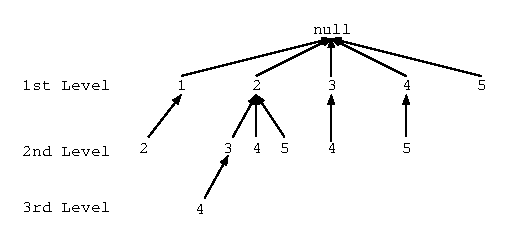
\includegraphics[height=2.5cm,width=7cm]{triefinal.eps}
\end{minipage}
}
\subfigure[Trie and candidate itemsets on the 2nd-level]{
\label{fig:trie:b}
\begin{minipage}[b]{.5\textwidth}
\centering
\includegraphics[height=2.5cm,width=7cm]{trie.eps}
\end{minipage}
}
\caption{Representing the trie in a relational table with the reference data type}
\end{figure}

{\renewcommand{\baselinestretch}{1}
\normalsize

\begin{algorithm}[!htb]
\begin{algorithmic}[1]

\STATE\kw{AGGREGATE} countset (bitem \kw{Int}, J \kw{Int}, $MinSup$ \kw{Int}, cands \kw{TABLE})\\
\STATE\{\hspace{.1cm}\kw{TABLE} previous(marked \kw{REF}(trie), Level \kw{Int})
 \kw{INDEX}(marked) \kw{MEMORY}; \\
\STATE\hspace{.3cm}\kw{TABLE} nextcands(cit \kw{Int}, trieref \kw{REF}(trie),
freqcount \kw{Int}) \kw{INDEX}(trieref) \kw{MEMORY};\\

\STATE\hspace{.3cm}\kw{INITIALIZE}: \kw{ITERATE}: \{ \\
\hspace{.6cm}\COMMENT{Intialize previous for a new transaction if bitem=0.}
\STATE\hspace{.6cm}\kw{DELETE} \kw{FROM} previous \kw{WHERE} bitem=0;\\
\STATE\hspace{.6cm}\kw{INSERT} \kw{INTO} previous \kw{VALUES} (null, 0) \kw{WHERE} bitem=0;\\
\hspace{.6cm}\COMMENT{Store supported frequent itemsets in previous}
\STATE\alglabel{algprev}\hspace{.6cm}\kw{INSERT} \kw{INTO} previous\\
\hspace{.9cm}\kw{SELECT} t.OID, p.Level+1 \kw{FROM} previous \kw{AS} p, trie \kw{AS} t\\
\hspace{.9cm}\kw{WHERE} t.itno=bitem \kw{AND} t.father=p.marked \kw{AND} p.Level$<$J-1;\\
\hspace{.6cm}\COMMENT{Count candidates that appear in the transaction}
\STATE\alglabel{algaddcount}\hspace{.6cm}\kw{UPDATE} cands \kw{SET} freqcount=freqcount+1 \\
\hspace{.9cm}\kw{WHERE} bitem $>$ 0 \kw{AND} c.cit=bitem\\
\hspace{1.3cm}\kw{AND} OID = (\kw{SELECT} c.OID \kw{FROM} previous \kw{AS} p, cands \kw{AS} c\\
\hspace{3.3cm}\kw{WHERE} p.Level=J-1 \kw{AND} c.trieref=p.marked);\\
\STATE\hspace{.2cm}\}\\

\STATE\hspace{.2cm}\kw{TERMINATE}: \{\hspace{.5cm}\\
% \STATE\hspace{1cm}\kw{DELETE} \kw{FROM} cands \kw{WHERE} freqcount $< MinSup$;\\
% \STATE\hspace{1cm}\kw{INSERT INTO} trie \kw{SELECT} cit,trieref \kw{FROM} cands;\\
\hspace{.6cm}\COMMENT{Derive  trie on level J and candidates on level J+1}
\STATE\alglabel{alggrow}\hspace{.6cm}\kw{INSERT} \kw{INTO} nextcands\\
\hspace{.9cm}\kw{SELECT} nextlevel (cit, trieref) \kw{FROM} cands \kw{WHERE} freqcount $\ge MinSup$ \kw{GROUP BY} trieref;\\
% \STATE\hspace{1cm}\kw{DELETE} \kw{FROM} cands;\\
% \STATE\hspace{1cm}\kw{INSERT} \kw{INTO} cands \kw{SELECT} * \kw{FROM} nextcands;\\
\hspace{.6cm}\COMMENT{Eliminate candidates by the anti-monotonicity}
\STATE\alglabel{alganti}\hspace{.6cm}\kw{INSERT} \kw{INTO} subitems \kw{VALUES}(null,0);\\
\STATE\hspace{.6cm}\kw{SELECT} checkset(cit, trieref), antimon(cit, trieref, J) \kw{FROM} nextcands; \\
\hspace{.6cm}\COMMENT{Ascend to level J+1 if cands not empty}
\STATE\alglabel{algrec}\hspace{.6cm}\kw{SELECT} countset (b.item, J+1, $MinSup$, nextcands) \\
\hspace{.9cm}\kw{FROM} (\kw{SELECT} count(*) \kw{AS} size \kw{FROM} nextcands) \kw{AS} c, baskets \kw{AS} b \kw{WHERE} c.size $>$0;\\
\hspace{.3cm}\}\\
\STATE\}
\end{algorithmic}
\caption{countset}
\label{alg:countset}
\end{algorithm}
The {\cw INITIALIZE} and {\cw ITERATE} routine of UDA {\bw countset}
is responsible for counting the occurrences of each candidate. As we
scan through each item in a transaction, we traverse the trie and
incrementally find all the itemsets that are supported by the
transaction, and we store the references to these itemsets in the {\bw
  previous} table (line~\algref{algprev}), which is initialized to
contain nothing but the root node at the beginning of each
transaction. On line~\algref{algaddcount}, the count of the candidate
is increased by 1 if the candidate itemset is supported by the
transaction. We will now continue with our example starting from the
trie in Figure~\ref{fig:trie:b}: after the first transaction,
$(2,3,4)$, is processed by {\bw countset}, table {\bw previous}
contains 4 nodes, namely the root, and nodes $2,3$, and $4$; also,
three candidate itemsets, $(2,3), (2,4)$, and $(3,4)$, have their
counts updated.

The {\cw TERMINATE} routine of {\bw countset} is responsible for
extending the trie to a new level.  On line~\algref{alggrow}, we call
{\bw nextlevel} to extend the trie to level $J$ by adding
candidates with a support no less than $MinSup$ to the trie.  The UDA {\bw
  nextlevel} also generates candidates on level $J+1$. Then, we apply
the anti-monotonic property to filter the candidates. This is
achieved by calling  {\bw checkset} and {\bw antimon} on
line~\algref{alganti}. Finally, on line~\algref{algrec}, we
recursively invoke {\bw countset} to extend the trie to level $J+1$
unless no new candidates are found.

{\renewcommand{\baselinestretch}{1}
\normalsize

\begin{algorithm}[!htb]
\begin{algorithmic}[1]
  \STATE\kw{TABLE} subitems(toid \kw{REF}(trie), level \kw{Int}) \kw{MEMORY};\\
  \COMMENT{extend the trie and return candidates on the new level}\\
  \STATE\kw{AGGREGATE} nextlevel(item \kw{Int}, ptrie \kw{REF}(trie)): (\kw{Int}, \kw{REF}(trie), \kw{Int})\\
  \STATE\{\hspace{.1cm}\kw{TABLE} previous(poid \kw{REF}(trie)) \kw{MEMORY};\\
  \STATE\hspace{.3cm}\kw{INITIALIZE}: \kw{ITERATE}: \{\\
  \STATE\alglabel{algext}\hspace{.6cm}\kw{INSERT} \kw{INTO} trie \kw{VALUES}(item, ptrie);\\
  \hspace{.6cm}\COMMENT{join with previously inserted itemsets and return them as next-level candidates}\\
  \STATE\hspace{.6cm}\kw{INSERT} \kw{INTO} \kw{RETURN} \kw{SELECT} item, previous.poid, 0 \kw{FROM} previous;\\
  \hspace{.6cm}\COMMENT{appending the newly-added to the previous
    table}
  \STATE\hspace{.6cm}\kw{INSERT} \kw{INTO} previous \\
  \hspace{.9cm}\kw{SELECT} trie.OID \kw{FROM} trie \kw{WHERE} trie.itno=item \kw{AND} trie.father=ptrie;\\
  \hspace{.3cm}\}\\
  \STATE\}\\
  \COMMENT{for each (J+1)-itemset, find its frequent subsets of size J}\\
  \STATE\kw{AGGREGATE} checkset (citem \kw{Int}, cref \kw{REF}(trie))\\
  \STATE\{\hspace{.2cm}\kw{INITIALIZE}: \kw{ITERATE}: \{\hspace{.5cm}\\
  \hspace{.6cm}\COMMENT {call checkset recursively}\\
  \STATE\hspace{.6cm}\kw{SELECT} checkset(f.itno, f.father) \kw{FROM} trie \kw{AS} f \kw{WHERE} cref$<>$null \kw{AND} f.OID=cref;\\
  \hspace{.6cm}\COMMENT {as we exit the recursion we expand subitems}\\
  \STATE\hspace{.6cm}\kw{INSERT} \kw{INTO} subitems \\
  \hspace{.9cm}\kw{SELECT} t.OID, s.level+1 \kw{FROM} subitems \kw{AS} s, trie \kw{AS} t\\
  \hspace{.9cm}\kw{WHERE} t.itno=citem \kw{AND} t.father=s.toid;\\
  \hspace{.3cm}\}\\
  \STATE\}\\
  \COMMENT{pruning using the anti-monotonic property}\\
  \STATE\kw{AGGREGATE} antimon(it \kw{Int}, aref \kw{REF}(trie), J \kw{Int})\\
  \STATE\{\hspace{.1cm}\kw{INITIALIZE}: \kw{ITERATE}: \{ \\
%  \hspace{.6cm}\COMMENT{eliminating a candidate if it has at least one subset of size J that is not frequent}\\
  \STATE\hspace{.6cm}\kw{DELETE} \kw{FROM} cands \\
  \hspace{.9cm}\kw{WHERE} cands.cit=it \kw{AND} trieref=aref\\
  \hspace{1.3cm}\kw{AND} J+1 $>$ (\kw{SELECT} count(*) \kw{FROM} subitems \kw{WHERE} subitems.level=J);\\
%  \hspace{.6cm}\COMMENT{reset the subitems table}\\
  \STATE\hspace{.6cm}\kw{DELETE} \kw{FROM} subitems \kw{WHERE} toid $<>$ null;\\
  \hspace{.2cm}\}
  \STATE\}
\end{algorithmic}
\caption{Supporting UDAs for Apriori}
\label{alg:support}
\end{algorithm}


\begin{figure}[htb!]
\subfigure[After invoking UDA {\bw nextlevel}]{
\label{fig:trie:c}
\begin{minipage}[b]{.5\textwidth}
\centering
\includegraphics[height=2.5cm,width=7cm]{trieprune.eps}
\end{minipage}
}
\subfigure[After invoking UDA {\bw checkset} and {\bw antimon}]{
\label{fig:trie:d}
\begin{minipage}[b]{.5\textwidth}
\centering
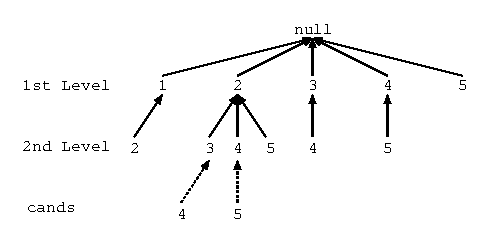
\includegraphics[height=2.5cm,width=7cm]{trieanti.eps}
\end{minipage}
}
\caption{Candidates generation and pruning}
\end{figure}

The UDA {\bw nextlevel} adds each qualified candidate onto the trie
(line~\algref{algext} in Algorithm~\ref{alg:support}).  It also
generates the next-level candidates by computing the self-join of the
newly added itemsets; this UDA is called with a {\cw GROUP BY} clause
to exclude candidates that do not share the same parent\footnote{A
  candidate resulting from self-joining itemsets that do not share the
  same parent is already included in the join result of
  itemsets that share the same parent, or will be eliminated by the
  anti-monotonic property.}.  The join operation is carried out
through the use of a temporary table called {\bw previous}, which
stores all the itemsets that appear ahead of the current itemset, and
they are joined with the current itemset to generate candidates on the
new level.  Figure~\ref{fig:trie:c} shows the result after {\bw
  nextlevel} is applied: qualified candidates in
Figure~\ref{fig:trie:b} become a new level of nodes in the trie, and a
new set of candidates are derived by self-joining the itemsets on
Level 2.

UDA {\bw checkset} and {\bw antimon} together implement the
anti-monotonic property for pruning. For each candidate itemset on
level $J+1$, {\bw checkset} traverses the trie to find all of its
sub-itemsets. According to the anti-monotonic property, a necessary
condition for a $(J+1)$-itemset to be a frequent itemset is that each
of its $J+1$ subsets is a frequent itemset. Thus, {\bw antimon}
eliminates those candidates that have fewer than $J+1$ frequent
itemsets of size $J$.  Figure~\ref{fig:trie:d} shows the result after
{\bw antimon} has eliminated candidate $(2,3,5)$ from
Figure~\ref{fig:trie:c}: $(2,3,5)$ cannot be a frequent itemset
because one of its subset, $(3,5)$, is not frequent.

As shown in Figure~\ref{fig:trie:a}, the
process on the sample dataset terminates at level 3.  At that point,
table {\bw trie} contain all the results, i.e., the frequent itemsets. \inv



\chapter{External Functions}
ATLaS supports both scalar external functions and table external
functions.

(For latest update, please refer to our website.)

\section{Scalar Functions}

To declare an external function to be dynamically loaded into ATLaS, we
use the following syntax:

\begin{verbatim}
external int ginif(a int) in 'gini.so';
\end{verbatim}

The above statement declares a UDF {\it ginif} which takes one
integer-type parameter and returns an integer result. This function is
supported by a shared library, 'gini.so'.

We can use C or any other language to create functions in shared
libraries. On a UNIX system, the following command compiles C source
code to dynamical libraries.

\begin{verbatim}
gcc -shared -o gini.so -fPIC gini.c
\end{verbatim}

Once defined, the UDF can be used in ATLaS. For instance:

\begin{verbatim}
select gini(a) from test;
\end{verbatim}

In order to dynamically load the library, the OS must be able to
find it. In UNIX, the OS searchs for the library in all the paths
specified by the environment variable LD\_LIBRARY\_PATH.

\section{Table Functions}
In much the same way, we can use external UDF as table functions.

For instance, we want to stream through the first K Fibonacci numbers.
It is not difficult to write a C function to generate the Fibonacci
numbers. The following ATLaS program demonstrates how to use such an
external table function.

\begin{verbatim}
external table (i int, f int) fib(k int) in 'tabf.so';

select t.i, t.f
from table (fib(10)) as t;
\end{verbatim}

In order to declare an external table function, we must use TABLE as
the return type. The above declaration indicates 'fib' is an external
function found in shared library 'tabf.so', and 'fib' returns a stream
of tubples (i,f), where f is the i-th Fibonacci number. Then, in the
following query, we stream through the first 10 Fibonacci numbers by
calling 'table (fib(10))'.

How do we implement a table function in C? Unlike stateless scalar
functions, table functions must keep their internal state between
calls. More specifically, the function must be able to: i) determine
the first call from subsequent calls; ii) tell the caller whether a
tuple is successfully returned; iii) use a mechanism to return tuples
to the caller. As an example, the following code implements function
'fib':

\begin{verbatim}
#include <db.h>

struct result {
  int a;
  int b;
};

int fib(int first_entry, struct result *tuple, int k)
{
  static int count;
  static int last;
  static int next;

  if (first_entry == 1) {
    count = 0;
    next=1;
    last=0;
  }
  if (count++ <k) {
    tuple->a = count;
    tuple->b = last;

    last = next;
    next = next+tuple->b;
    return 0;
  } else {
    return DB_NOTFOUND;
  }
}
\end{verbatim}

In addition to the arguments (here is 'k') passed to the table
function, we have 2 extra arguments: i) $first\_entry$, if
first\_entry=1 then it is the first call; ii) tuple, which is a
pointer to a structure where results are to be stored. External
table functions always return an integer value, 0 if successful,
DB\_NOTFOUND otherwise.

A possible use of table functions is to scan file system data, and
return results to the database system after filtering. Our test
indicates that on a linux system, external table functions accessing
file system data is almost 100 times faster than accessing the same
data in the Berkeley DB format.


\section{Built-in Aggregates and Functions}
ATLaS supports the standard builtin aggregates: {\bf min()}, {\bf
  max()}, {\bf sum()}, {\bf avg()}, and {\bf count()}.

ATLaS supports the following builtin functions: (they are being added
constantly.)

\begin{itemize}
\item {\bf srand(INT) : INT} \\
  The srand() function sets its argument as the seed for a new
  sequence of pseudo-random integers to be returned by rand().  These
  sequences are repeatable by calling srand() with the same seed
  value. srand() always returns 0.

\item {\bf rand() : REAL} \\
  The rand() function returns a pseudo-random real between 0 and 1.
  The following code set 10 as a random seed, and displays two random
  values.
\begin{verbatim}
    VALUES(srand(10));

    VALUES(rand(), rand());
\end{verbatim}

\item {\bf sqrt(REAL) : REAL}\\
  The sqrt(x) function returns the non-negative square root of x.  \\

\item {\bf timeofday() : CHAR(20)}\\
  The gettimeofday function gets the system's notion of the current
  time. The current time is expressed in elapsed seconds and
  microseconds since 00:00 Universal Coordinated Time, January 1,
  1970. It returns a string in the form of x'y'', where x is the
  seconds and y is the microseconds. This function is maily used to
  measure the performance of ATLaS queries, as in the following example:

\begin{verbatim}
    INSERT INTO stdout VALUES(timeofday());

    ... some ATLaS queries ...

    INSERT INTO stdout VALUES(timeofday());
\end{verbatim}
\end{itemize}

\begin{thebibliography}{aaaa}

\bibitem{agg94} R. Agrawal, R. Srikant.
\newblock ``Fast Algorithms for Mining Association Rules''.
\newblock In {\em VLDB'94}.


\bibitem{hellerstein} J.~M. Hellerstein, P.~J. Haas, H.~J.
Wang.  \newblock ``Online Aggregation''.  \newblock {\em SIGMOD,
  1997}.


\bibitem{cachemine} S. Sarawagi, S. Thomas, R.  Agrawal,
\newblock ``Integrating Association Rule Mining with Relational
Database Systems: Alternatives and Implications''. In \newblock {\em
  SIGMOD, 1998}.


\bibitem{sprint} J. C. Shafer, R. Agrawal, M. Mehta, \newblock
``SPRINT: A Scalable Parallel Classifier for Data Mining,"
\newblock In {\em VLDB 1996}.

\bibitem{berkeleydb} Sleepycat Software, ``The Berkeley Database
(Berkeley DB)'', \newblock http://www.sleepycat.com.

\bibitem{vldb2k}
H. Wang and C. Zaniolo:
\newblock Using SQL to Build New Aggregates and Extenders for Object-Relational
Systems.
\newblock VLDB 2000.

\bibitem{ads}
Carlo Zaniolo, Stefano Ceri, Christos Faloutsos,
Richard T. Snodgrass, V. S. Subrahmanian, Roberto Zicari:
Advanced Database Systems. Morgan Kaufmann 1997, ISBN 1-55860-443-X.
\end{thebibliography}

%\input{issues}
\end{document}
